\documentclass{beamer}
    \mode<presentation> {
    \usetheme{Montpellier}
    \usecolortheme{beaver}
    
    %\setbeamertemplate{footline} % To remove the footer line in all slides uncomment this line
    \setbeamertemplate{footline}[page number] % To replace the footer line in all slides with a simple slide count uncomment this line
    
    \setbeamertemplate{navigation symbols}{} % To remove the navigation symbols from the bottom of all slides uncomment this line
    }
    
    \usepackage{graphicx} % Allows including images
    \usepackage{booktabs} % Allows the use of \toprule, \midrule and \bottomrule in tables
    \usepackage {tikz}
    \usetikzlibrary {positioning}
    \graphicspath {{media/}}
    %----------------------------------------------------------------------------------------
    %	TITLE PAGE
    %----------------------------------------------------------------------------------------
    
    \title[PPER]{Project Networks and Percept-Plan-Execute Loop \\ to the rescue}
    
    \institute[Septimal Mind]
    {
    Septimal Mind Ltd.\\
    \medskip
    \textit{team@7mind.io}
    }
    \date{\today}
    
    \begin{document}
    
    \begin{frame}
    \titlepage
    \end{frame}
    
    \begin{frame}
    \frametitle{Overview} % Table of contents slide, comment this block out to remove it
    \tableofcontents % Throughout your presentation, if you choose to use \section{} and \subsection{} commands, these will automatically be printed on this slide as an overview of your presentation
    \end{frame}
    
\section{What is this all about?}
\subsection{The Problem}

\begin{frame}
    \frametitle{What are we doing?}
    \begin{itemize}
        \item We are building systems   
          \begin{itemize}
            \item Complex ones
          \end{itemize}
        \item We need to deliver our work in time and avoid fuckups
          \begin{itemize}
            \item But we also want to have a life
          \end{itemize}        
        \item So we are aiming for productivity

        \item What makes our life hard?
        \begin{itemize}
            \item Complexity.
          \end{itemize}        
    \end{itemize}    
 \end{frame}

\begin{frame}
    \frametitle{Where complexity lies?}

    Everywhere in the SDLC:
    \begin{itemize}
        \item Domain analysis: we need to understant The Problem first
        \item Initial formalization: make it fairly formal
        \item Design: it's hard to make Our Things maintainable and viable
        \item Development
        \begin{itemize}
            \item State
            \item Coupling
            \item Tests
            \item Protocols, especially asynchronous
        \end{itemize}     
        \item Integration
        \item Delivery
        \item Maintenance
    \end{itemize}

\dots and there are thousands of opinions on How To Do The Things
%    In order to build something we need to
%    understand the problem (analyse our Domain)
%    come up with the solution
%    formalise it at a level enough to start expressing it with a code

\end{frame}

\begin{frame}
    \frametitle{So what?}

    We are going to talk about Domain Anaylisys and understand how to 
    do things better.

    \begin{itemize}
        \item Recently we've discussed Event Storming as a way to get some grip on the domain
        \item We have Mindmaps for the same purpose
        \item And we have Flowcharts as a ``simplified'' formal definition
        \item And don't forget about UML (does anyone like it as a \textit{modeling} tool?)
        \item and there are many other approaches
    \end{itemize}
    

    but\dots
\end{frame}


\subsection{What's wrong with everything?}

\begin{frame}
    \frametitle{The Hell}
    What to do in case our domain is \textit{inconceivable}?

    We may have: 
    \begin{itemize}
        \item thousands of entities we need to represent
        \item thousands of events
        \item complex flows 
        \item sequential and parallel subflows
        \item undecidability
    \end{itemize}

    Examples:
    \begin{itemize}
        \item American healthcare: enormous amounts of entities, complex protocols involving a lot of human interaction
        \item Cluster orchestration: fairly low amount of entities but protocols are deadly complex, too much uncertainty and undecidability
    \end{itemize}
\end{frame}

\begin{frame}
    \frametitle{The Hell: flowcharts}
    
    \begin{figure}
        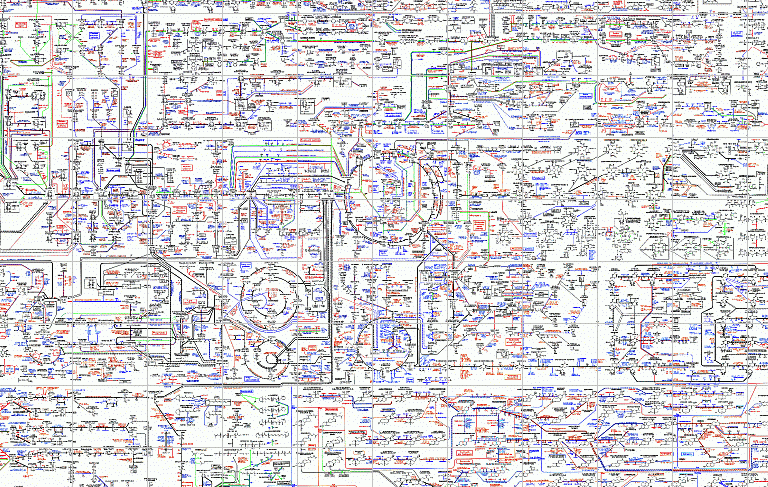
\includegraphics[width=\textwidth]{media/flowshit}
    \end{figure}
\end{frame}

\begin{frame}
    \frametitle{The Hell: flowcharts}
    
    \begin{itemize}
        \item They grow fast and it's easy to make them too complex to be useful
        \item Flowcharts are not hierarchical 
        \item They allow us to create loops and conditions, so they are Turing-complete. Better write code.
    \end{itemize}
\end{frame}

\begin{frame}
    \frametitle{The Hell: events}
    
    \begin{figure}
        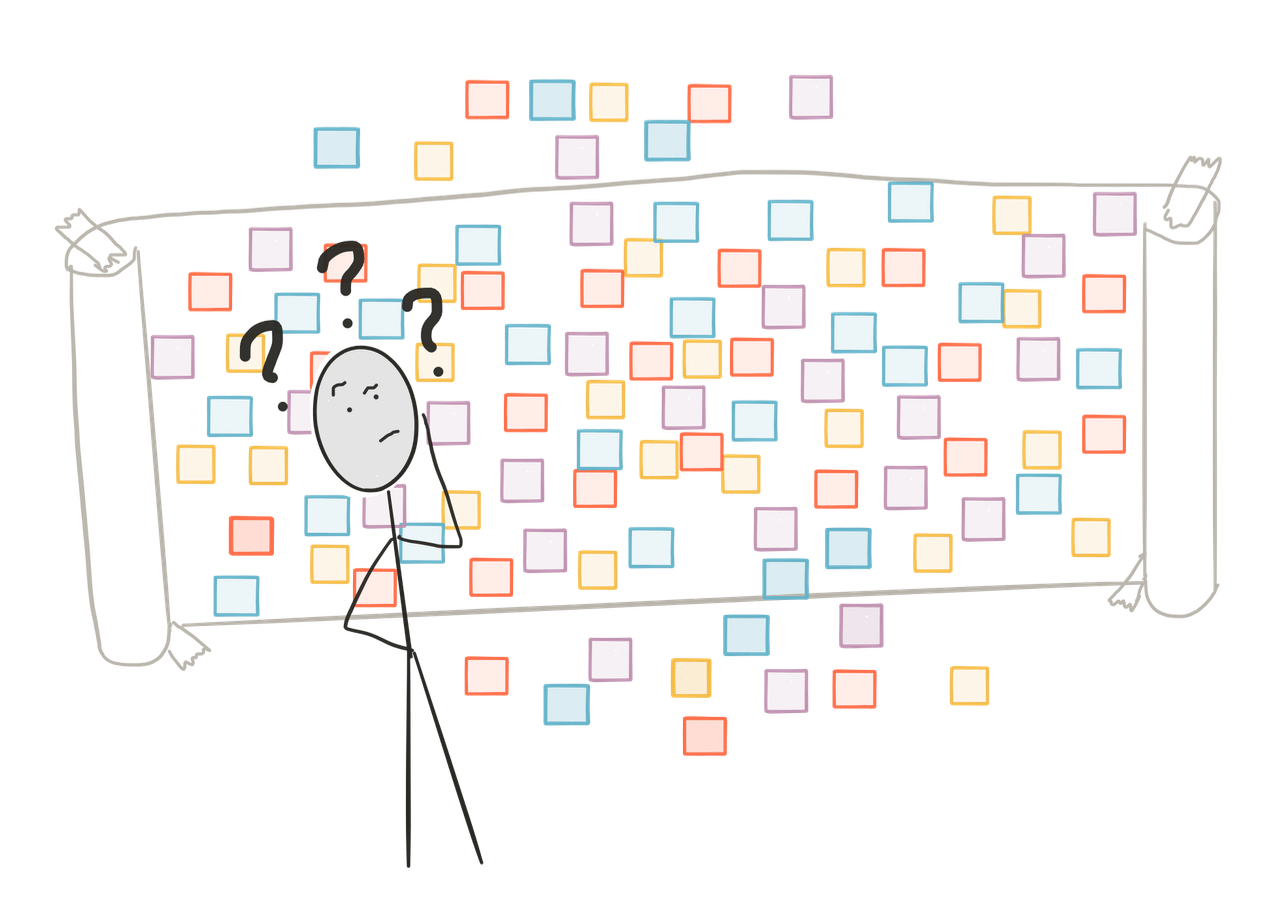
\includegraphics[width=\textwidth]{media/eventstorming}
    \end{figure}
    
\end{frame}

\begin{frame}
    \frametitle{The Hell: events}
    
    \begin{itemize}
        \item There is a duality of Entities and Events
        \item Event Storming board is flat
        \item These hundreds of sticky notes are hard to handle
        \item We still need Turing-complete formalisms
    \end{itemize}
\end{frame}

\section{Some interesting stuff}
\subsection{A bit of boring definitions}

\begin{frame}
    \frametitle{Project networks}
    \begin{itemize}
        \item Usually it's not so hard to express the Happy Path.
        \item It's hard to handle cornercases, branches, etc
        \item \textit{Project network} is a DAG where nodes are actions to do and edges are dependencies
        \begin{itemize}
            \item Natural way to express parallelism         
        \end{itemize}            
    \end{itemize}    
\end{frame}

\begin{frame}
    \frametitle{Example: build a house}
    \begin{figure}
        \includegraphics[width=\textwidth]{media/pn-house}
    \end{figure}
\end{frame}


\begin{frame}
    \frametitle{Example: hiring process}
    \begin{figure}
        \includegraphics[width=\textwidth]{media/pn-hiring-top}
    \end{figure}
\end{frame}

\begin{frame}
    \frametitle{Example: hiring process step}
    \begin{figure}
        \includegraphics[width=\textwidth]{media/pn-hiring-step}
    \end{figure}
\end{frame}


\begin{frame}
    \frametitle{Project networks: how to use}
    \begin{itemize}
        \item Let's represent our flows as Project Networks
        \item Nodes would stand for actions to do, \textit{verbs}
        \item Let's call a Node \textit{trivial} in case it represents an atomic action
        \item Let's call a Node \textit{complex} in case it represents a complex action
    \end{itemize}
Important to remember:
    \begin{itemize}
        \item A Complex Node can be represented as another, \textit{nested} Project Network
        \item We can build a hierarchy of abstractions
        \item Each abstraction level is described by Verbs and Flows composable out of them
        \item Verbs available at a level would form a DSL
        \item Each subordered level should have higher detailization and locality
    \end{itemize}
\end{frame}

\begin{frame}
    \frametitle{Case Management}
    A boring definition:
    
    \begin{itemize}
        \item ``\textit A {Case} is a collection of information and coordinated activities by knowledge workers or case workers''
        \item ``Represents an entity that the organization must process and it is sometimes identified by having a subject''
    \end{itemize}
\end{frame}

\begin{frame}
    \frametitle{Case Management}

    Common organizational pattern:

    \begin{itemize}
        \item We have an abstract context named \textit{Case}
        \item A case consisting of \textit{Facts} --- abstract datums
        \item Initially a case consists of an \textit{Problem} (input) and a \textit{Goal}
        \item We have a nondeterministic sequence of \textit{Phases} which should allow us to achieve the Goal
        \item Each Phase may add some new Facts into the case
        \item Each Phase can be executed by an idependent actor
        \item Case Lifecycle is governed by coordinating actor named \textit{Case Manager}
        \item The context is considered alive by the Case Manager unless the Goal is reached
    \end{itemize}
\end{frame}

\begin{frame}
    \frametitle{Case Management}
    
    \begin{figure}
        \includegraphics[width=\textwidth]{media/case-management}
    \end{figure}
\end{frame}

\begin{frame}
    \frametitle{Viable System Model}
    
\begin{itemize}
    \item An organizational model of an animal neural system
    \item Introduced by Stafford Beer
    \item Proposes a way to implement \textit{homeostasis} in an abstract system
    \item Intended to deal with complexity and uncertainty  
\end{itemize}

Key points:
\begin{itemize}
    \item Algedonic regulation
    \item Hierarchy of interacting subsystems
    \item Levels are local autonomic
    \item Metalanguage stack
    \item Variety increases top-down and decreases bottom-up: 
          we are operating a limited set of high-level abstractions on top level 
          and many low-level abstractions at the bottom level
\end{itemize}
\end{frame}

\section{PPER loop and The Ultimate Machine}
\subsection{The Pattern}
\begin{frame}
    \frametitle{How not to get crazy on domain analysis}  
\begin{itemize}
    \item Let's represent our domain as a set of Cases
    \begin{itemize}
        \item Works well for many, many real processes
        \item Not for every though. Not a silver bullet.         
    \end{itemize}   
    \item Let's draw Project Networks for each case
    \item Don't try to cover all the cornercases, concentrate on primary flows 
    \item Try to keep vocabulary tiny
    \item In case you need a branch try to create a sub-network
\end{itemize}
\end{frame}

\begin{frame}
    \frametitle{How to make it formal enough to use?}  
    
\begin{itemize}
    \item Okay, this may be useful for getting grip on our domain,
    \item But now to turn it into the code?
\end{itemize}
\end{frame}

\begin{frame}
    \frametitle{PPER Loop}  
    
    A very generic and a very important pattern:
\begin{enumerate}
    \item Acquire data from the outer world (\textit{Percept})
    \item Produce a Project Network, \textit{Plan}. 
          It may be incomplete, it should allow us to progress (\textit{Plan})
          \begin{itemize}
            \item Plan is a DAG, remember?       
          \end{itemize} 
    \item Execute the Plan (\textit{Execute}). 
    \begin{itemize}
        \item Perform the steps of the Plan
        \item Mark your Plan nodes according to the results of their execution    
        \item Let's call marked plan as \textit{Trace}
      \end{itemize} 
    \item Go to step 1 unless termination criteria reached (\textit{Repeat})
\end{enumerate}
\end{frame}

\begin{frame}
    \frametitle{PPER Loop}
    
    \begin{figure}
        \includegraphics[width=\textwidth]{media/pper}
    \end{figure}
\end{frame}

\begin{frame}
    \frametitle{Parts for The Ultimate Machine}  
\begin{enumerate}
    \item \textit{Sensor} or \textit{Afferent Channel} is a data source. Allows us to get some state from the outer world.
    \item \textit{Planner} an abstract entity taking Sensor Data, Previous Plan and Previous Trace and producing new Plan
    \item \textit{Executor} or \textit{Efferent Channel} is an entity able to change outer world and get a result
\end{enumerate}
\end{frame}

\subsection{The Ultimate Machine}
\begin{frame}
    \frametitle{Let's put things together}  
    We may imagine an abstract machine supporting PPER loop:
\begin{enumerate}
    \item A Specification is a set of $(name, type)$ pairs. $S = [(name, type)]$
    \item A Verb is a name plus input specification plus output specification. $v = \{name, In_v, Out_v\}$
    \item A language is: set of verbs, bindings for executors for each verb, planner, sensors, goal specification, problem specification.
         $L = \{planner_L, E_L, S_L, V_L, g_L, p_L\}$
    \item So we have a hierarchy of abstract incomplete languages, \textit{Metalanguage} $ML = [L_1, \dots L_n]$
\end{enumerate}
\end{frame}

\begin{frame}
    \frametitle{Let's put things together}  
\begin{enumerate}
    \item Let's isolate each PPER loop in a separate stackframe
    \item Each stackframe contains Context, Sensors, Planner, Executors, current Plan, current Trace, previous Trace, previous Plan and array of subordered frames
    \item In fact it's not a stack, it's a tree
    \item When an Executor starts working on a non-trivial Step we should create a new stackframe
\end{enumerate}
\end{frame}

\begin{frame}
    \frametitle{The Ultimate Machine}
    
    \begin{figure}
        \includegraphics[width=\textwidth]{media/machine-stack}
    \end{figure}
\end{frame}

\begin{frame}
    \frametitle{What do we have now?}  
\begin{itemize}
    \item All the entities are stateless, the state is held in the machine's stack.
    \item Turing Complete but \textit{pure} Planners.
    \item Turing Incomplete Plans are easy to analyse.
    \item \textbf{Effect Separation} as a part of our design.
    \item Arbitrary planning strategies  
    \item Testability: Planning is repeatable so easy to test.
    \item Perfect simulations.
    \item Introspectability: it's easy to visualize even very complex processes.
    \item Traceability: we may record all the history stack states.
    \item Portable State: machine state is easy to serialize, restore, explore offline. 
    \item Parallelism
\end{itemize}
\end{frame}

\begin{frame}
    \frametitle{Let's go further}  
\begin{itemize}
    \item Planning may be \textbf{delegated to a human}!
    \item So may Execution
    \item We may add a UI with a task queue (like Amazon Mechanical Turk)
    \begin{itemize}
        \item Perfect Business Process Management solution
        \item Perfect HRMS
        \item Gamification
        \item Onboarding
        \item Plans, produced by a human, may be reused
        \item ML, Data Mining\dots
    \end{itemize}   
\end{itemize}
\end{frame}

\begin{frame}
    \frametitle{Applications}  
    Many problems related to Operations Research and requiring dynamic planning
\begin{itemize}
    \item Homeostasis problems: orchestration, robotics, adaptive/viable systems\dots
    \item Project Planning and dynamic business flows: HRM, CRM, Project Management
    \item Build tools, DI frameworks\dots 
    \begin{itemize}
        \item I have implemented a DI framework, exploiting the PPER principle :)
    \end{itemize}   
\end{itemize}
\end{frame}


\begin{frame}
    \frametitle{How to plan?}  
\begin{itemize}
    \item An endless subject.
    \item Easier than usual because of the separation
    \item Any approach you wish: ML, Constraint solving, Genetic Algorithms\dots
    \item An interesting idea: to make planners typesafe and prove safety in compile time
    \item Prolog and other constraint solvers would work great  
\end{itemize}
\end{frame}

\section{What else?}
\begin{frame}
    \frametitle{More interesting stuff}
    
    The author would be happy to make more presentations 
    regarding some projects he is working on right now:

    \begin{itemize}
        \item Staged Generative DI framework. (Best one, you wouldn't need Guice anymore)
        \item Data modeling and interface definition language. (Forget about GRPC/Protobuf)
        \item Structural logging (and how to make it free)
    \end{itemize}
\end{frame}

\begin{frame}
    \frametitle{Thank you for your attention}

    \begin{center}
      We're looking for clients, contributors, adopters and colleagues ;)
    \end{center}

    About the author:
    \begin{itemize}
        \item coding for 18 years, 10 years of hands-on commercial engineering experience,
        \item has been leading a cluster orchestration team in Yandex, ``the Russian Google'',
        \item implemented ``\textit{Interstellar Spaceship}'' -- an orchestration solution to manage 50K+ physical machines across 6 datacenters,
        \item Owns an Irish R\&D company, https://7mind.io,
        \item Contacts: team@7mind.io,
        \item Github: https://github.com/pshirshov
    \end{itemize}
\end{frame}

\end{document} 